\section{An exact two-bounce boundary response in Lovelock gravity}
\label{sec:lovelock}

The Einstein calculation in section~\ref{sec:einstein-poles} isolates a high-frequency sector. We now solve the boundary-value problem and continue the full correlator in an exactly soluble Lovelock background.

\subsection{Background and scalar reduction}

Consider Lovelock gravity of order \(K\geq2\) with a unique AdS vacuum of multiplicity \(K\) and unit AdS radius \cite{Crisostomo:2000,Cai:2001,BravoGaete:2013}. Set the boundary dimension to \(d=4K\). With flat transverse sections and unit horizon radius, the static vacuum first integral is
\begin{equation}
 \left(1-\frac{f(r)}{r^2}\right)^K=r^{-d}.
\end{equation}
On the branch with \(1-f/r^2>0\), this gives \(f(r)=r^2-r^{-2}\) in bulk dimension \(4K+1\). The background metric is of the form \eqref{eq:metric}, with this new \(f\). Its regular horizon has \(\beta=\pi\), since \(f'(1)=4\). At \(r=0\) its scalar curvature is
\begin{equation}
 {\cal R}=-d(d+1)+(d-3)(d-4)r^{-4}.
\end{equation}
The divergence and \(g^{rr}<0\) inside the horizon give a spacelike curvature singularity. The radial optical geometry is that of the Einstein AdS\(_5\) brane because the two lapse functions coincide. The higher-dimensional transverse geometry and the scalar field theory below are different.

Take a zero-momentum scalar with effective mass \(m_{\rm eff}^2=m_0^2+\xi{\cal R}\) and time dependence \(e^{-\ii\omega t}\). For \(a=(d-2)/2\), choose
\begin{equation}
 \xi=\frac{a(a-2)}{(d-3)(d-4)},\qquad
 m_0^2=-a(a+2)+\xi d(d+1).
 \label{eq:tuned-mass}
\end{equation}
For example, in \(D=d+1=9\), \(\xi=3/20\) and \(m_0^2=-21/5\). The asymptotic effective mass is \(1-d^2/4\), which is above the Breitenlohner--Freedman bound. We use standard quantization, with \(\Delta=d/2+1\). On substituting \(\phi=r^{-a}A\) into the scalar equation, the coefficient of \(A'\) is \(f'/f+1/r\), and the non-frequency part of the coefficient of \(A\) vanishes because
\begin{equation}
 m_{\rm eff}^2=-a^2 f/r^2-a f'/r=-a(a+2)+a(a-2)r^{-4}.
\end{equation}
The reduced equation is \((r f A')'+\omega^2 r A/f=0\), with primes here denoting \(r\) derivatives. This is the equation for the transverse current in the known Einstein AdS\(_5\) example \cite{Kovtun:2005,AfkhamiJeddi:2025}. Here its solution gives a scalar boundary response in higher dimension through \eqref{eq:tuned-mass}.

\subsection{Ingoing solution and spectral density}

Define \(z=\operatorname{artanh}(r^{-2})\) and \(w=\omega/2\). The exterior \(1<r<\infty\) maps to \(0<z<\infty\) and \(r f\,\dd z/\dd r=-2\). The reduced equation is
\begin{equation}
 A_{zz}+w^2\coth(z) A=0.
 \label{eq:lovelock-z}
\end{equation}
The retarded horizon condition is \(A\propto e^{+\ii wz}\) as \(z\to\infty\). A source-free mode vanishes at \(z=0\). For \({\rm Im}\,\omega>0\) the ingoing solution decays at infinity, and integration by parts for a putative source-free mode would require \(\int |A_z|^2\dd z=w^2\int \coth(z)|A|^2\dd z\). This excludes such a mode in the upper half-plane.

To obtain the response, put \(v=\coth z\), \(s=(1+\ii)w/2\), and \(y=(1-v)/2\). Factoring the exponents at \(v=\pm1\) gives the hypergeometric solution that is ingoing at the real horizon,
\begin{equation}
 A_{\rm in}=(v-1)^{-\ii w/2}(v+1)^{-w/2}
 {}_2F_1(-s,1-s;1-\ii w;y).
\end{equation}
The ingoing amplitude has modulus \(2^{-w/2}\) for real \(w>0\). At the boundary \(v\to\infty\), the leading hypergeometric connection term gives the source
\begin{equation}
 A^{(0)}=2^{-s}\frac{\Gamma(1-\ii w)}
                  {\Gamma(1-s)\Gamma(1+\bar s)}.
\end{equation}
The logarithmic subleading term does not enter the conserved flux. The original scalar flux reduces to that of \(A\), since
\begin{equation}
 r^{d-1} f\,{\rm Im}(\bar\phi\,\partial_r\phi)
 =r f\,{\rm Im}(\bar A\,\partial_r A)
 =-2\,{\rm Im}(\bar A\,A_z).
\end{equation}
Thus the ingoing flux magnitude, divided by \(2|A^{(0)}|^2\), is
\begin{equation}
 w\frac{|\Gamma(1-s)\Gamma(1+\bar s)|^2}{|\Gamma(1-\ii w)|^2}
 =\pi w^2\frac{\sinh(\pi w)}{\cosh(\pi w)-\cos(\pi w)}.
\end{equation}
Here the gamma reflection identity gives the last expression. In pure AdS, the same reduced probe equation has unit-source solution \((\ii\pi/2)(\omega/r)H_1^{(1)}(\omega/r)\) and half-flux \(\pi w^2\). Consequently the exact spectral density, normalized by its positive-frequency vacuum value, is
\begin{equation}
 \frac{\rho(\omega)}{\rho_{\rm vac}(\omega)}
 =\frac{\sinh(\pi w)}{\cosh(\pi w)-\cos(\pi w)}
 =1+2\sum_{n=1}^{\infty}e^{-n\pi w}\cos(n\pi w),
 \qquad w=\omega/2>0 .
 \label{eq:lovelock-spectral}
\end{equation}
The radial null round trip has time \(T_*=\frac{\pi}{2}(1-\ii)\), with partner \(-T_*^*\), using the same horizon prescription as \eqref{eq:tstar}. The \(n\)-th term in \eqref{eq:lovelock-spectral} contains exactly the phases \(e^{-\ii n\omega T_*}\) and \(e^{+\ii n\omega T_*^*}\). In particular the two-bounce contribution is
\begin{equation}
 \left.\frac{\delta\rho}{\rho_{\rm vac}}\right|_{n=2}
   =2 e^{-\pi\omega}\cos(\pi\omega).
 \label{eq:lovelock-twobounce}
\end{equation}
These are repeated trips with finite time per reflection. The contractible local cycles of section~\ref{sec:cycles} do not enter the derivation of \eqref{eq:lovelock-spectral}.

\begin{table}[t]
 \centering\small
 \begin{tabular}{cccc}
 \hline
 \(\omega\) & numerical residual after \(n=1\) & exact \(n=2\) term & bound on \(n\geq3\)\\
 \hline
 2.0 & +0.00358017 & +0.00373489 & +0.00016869 \\
2.8 & -0.00024173 & -0.00024476 & +0.00000377 \\
3.6 & +0.00000755 & +0.00000757 & +0.00000009 \\
\hline

 \end{tabular}
 \caption{Direct radial integration of the original scalar in bulk dimension
 \(D=9\), after subtracting the vacuum and the first reflection from
 \(\rho/\rho_{\rm vac}\). The bound is \(2e^{-3\pi w}/(1-e^{-\pi w})\).}
 \label{tab:lovelock}
\end{table}

For Table~\ref{tab:lovelock} we integrate the nonminimally coupled equation for \(\phi\), without using its hypergeometric solution. We start with ingoing wave data at a large value of \(z\) and read the source from \(r^a\phi\) at small \(z\). Halving the integration step and moving both cutoffs checks the convergence. For \(D=9\) and \(13\) the normalized densities agree with \eqref{eq:lovelock-spectral} to absolute error below \(7\times10^{-11}\) at the tested frequencies. This resolves the two-bounce term and its change of sign.

\subsection{The two-bounce poles in complex time}

The spectral result also determines the continued Wightman correlator. Use \(\tau=\beta/2\) in this subsection and \(\rho_{\rm vac}(\omega)=C\omega^2\) for \(\omega>0\), with \(C\) a positive normalization. The thermal relation \(G^>(\omega)=\rho(\omega)/(1-e^{-\beta\omega})\) gives
\begin{equation}
 G^>(\omega)=C\omega^2\sum_{j,k\geq0}
  e^{-(j+k)\tau\omega+\ii(j-k)\tau\omega},\qquad \omega>0 .
\end{equation}
For negative frequency use \(G^>(-\omega)=e^{-\beta\omega}G^>(\omega)\) with \(\omega>0\). Fourier transforming with \(e^{-\ii\omega t}\) in the thermal strip \(-\beta<{\rm Im}\,t<0\) gives the meromorphic continuation
\begin{align}
 G^>(t)=\frac{C}{\pi}\sum_{j,k\geq0}\Big\{&
 \big[(j+k)\tau+\ii(t-(j-k)\tau)\big]^{-3}\notag\\
 &+\big[(j+k+2)\tau-\ii(t+(j-k)\tau)\big]^{-3}\Big\}.
 \label{eq:lovelock-time}
\end{align}
Indeed, at fixed \(j+k=N\) there are \(N+1\) terms and the two denominators grow linearly in \(N\), so the sum converges locally uniformly away from its poles. In particular, the terms \((j,k)=(2,0),(0,2)\) in the first line give third-order poles at \(t=\pm\beta+\ii\beta\). The mixed term \((1,1)\) at \(t=\ii\beta\) has zero real displacement and is a thermal image. Figure~\ref{fig:poles} shows the positive and negative frequency lattices and the physical thermal strip between them.

\begin{figure}[t]
\centering
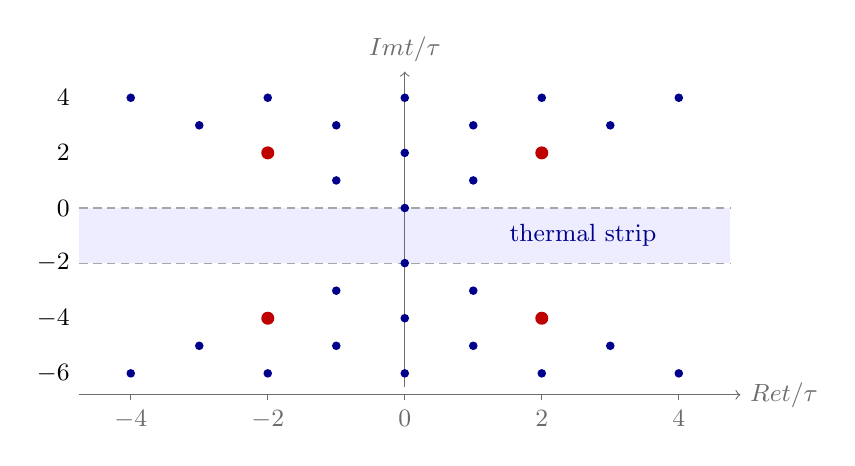
\begin{tikzpicture}[x=0.87cm,y=0.35cm, every node/.style={font=\small}]
 \fill[blue!7] (-4.75,-2) rectangle (4.75,0);
 \draw[gray!70,densely dashed] (-4.75,0) -- (4.75,0);
 \draw[gray!70,densely dashed] (-4.75,-2) -- (4.75,-2);
 \draw[->,gray!85!black] (0,-6.5) -- (0,4.95)
    node[above] {\(\operatorname{Im}t/\tau\)};
 \draw[->,gray!85!black] (-4.75,-6.78) -- (4.9,-6.78)
    node[right] {\(\operatorname{Re}t/\tau\)};
 \foreach \x in {-4,-2,0,2,4} {
   \draw[gray!85!black] (\x,-6.78) -- (\x,-6.98)
      node[below] {\(\x\)};
 }
 \foreach \y in {-6,-4,-2,0,2,4} {
   \node[left] at (-4.75,\y) {\(\y\)};
 }
 \node[blue!55!black] at (2.6,-1) {thermal strip};
 \foreach \n in {0,...,4} {
   \foreach \k in {0,...,\n} {
     \fill[blue!55!black] ({\n-2*\k},\n) circle[radius=1.55pt];
     \fill[blue!55!black] ({-\n+2*\k},{-\n-2}) circle[radius=1.55pt];
   }
 }
 \foreach \x in {-2,2} {
   \fill[red!75!black] (\x,2) circle[radius=2.35pt];
   \fill[red!75!black] (\x,-4) circle[radius=2.35pt];
 }
\end{tikzpicture}
\caption{Pole lattice of the Lovelock scalar Wightman function in units of
 \(\tau=\beta/2\). The red points are the two-bounce pair and its image
 under \(t\mapsto-t-\ii\beta\). The shaded open thermal strip contains
 no poles.}
\label{fig:poles}
\end{figure}


\subsection{Mass dependence of the exact reflection series}
\label{sec:detuning}

The exact solution persists after varying the bare mass at fixed curvature coupling \(\xi\). Add \(\nu^2-1\) to \(m_0^2\) in \eqref{eq:tuned-mass}, with \(\nu>0\). The boundary weight is now \(\Delta=d/2+\nu\) in standard quantization. The optical geometry is unchanged. In \(v=r^2=\coth z\), the reduced scalar obeys
\begin{equation}
 A_{vv}+\frac{2v}{v^2-1}A_v+
 \left[\frac{w^2 v}{(v^2-1)^2}-\frac{\nu^2-1}{4(v^2-1)}\right]A=0 .
 \label{eq:detune-v}
\end{equation}
It still has three regular singular points. With \(h=(1+\nu)/2\), \(s_\pm=(1\pm\ii)w/2\), and \(y=(1-v)/2\), the ingoing hypergeometric parameters become
\begin{equation}
 a_0=1-h-s_+,\qquad b_0=h-s_+,\qquad c_0=1-\ii w .
\end{equation}
The horizon prefactor is unchanged. At infinity the two powers of \(A\) are \(r^{\nu-1}\) and \(r^{-\nu-1}\). For \(\nu\notin\mathbb Z\), the ratio of their coefficients, with response over source, is
\begin{equation}
 2^\nu\frac{\Gamma(-\nu)}{\Gamma(\nu)}
 \frac{\Gamma(h-s_+)\Gamma(h+s_-)}
 {\Gamma(1-h-s_+)\Gamma(1-h+s_-)} .
 \label{eq:detuned-g}
\end{equation}
For real \(w>0\), the half-flux divided by the squared source is
\begin{equation}
 {\cal J}_\nu=
 w\,2^{\nu-1}
 \frac{|\Gamma(h-s_+)\Gamma(h+s_-)|^2}
      {|\Gamma(1-\ii w)|^2\Gamma(\nu)^2}.
\end{equation}
The source has no zeros for \({\rm Im}\,\omega>0\): the potential zeros from the reciprocal gamma factors occur at \(\omega=\pm 2(h+n)-2\ii(h+n)\) with \(n\geq0\).
This flux is finite also at integer \(\nu\), where the boundary expansion has logarithms. The unit-source pure-AdS solution is \(A=(\ii\pi w^\nu/\Gamma(\nu))\,r^{-1}H^{(1)}_\nu(\omega/r)\), giving \({\cal J}_{\rm vac}=\pi w^{2\nu}/\Gamma(\nu)^2\). The gamma reflection identity then yields
\begin{align}
 \frac{\rho_\nu}{\rho_{\rm vac}}
 &=P_\nu(w)\frac{\sinh(\pi w)}{\cosh(\pi w)-\cos\theta},
 &\theta&=\pi\big(w-\nu-1\big),\notag\\
 P_\nu(w)
 &=\frac{1}{(w^2/2)^\nu}
     \left|\frac{\Gamma(h+s_+)}{\Gamma(1-h+s_+)}\right|^2.
 \label{eq:detuned-spectrum}
\end{align}
After dividing by the exact envelope \(P_\nu\), the \(n\)-th reflection harmonic is \(2e^{-n\pi w}\cos(n\theta)\). The damping time per reflection is independent of \(\nu\), whereas the phase varies with the probe. Equation~\eqref{eq:detuned-spectrum} is a factorization of the full positive-frequency spectrum. For noninteger \(\nu\), identifying its geometric factor with the complete beyond-all-orders expansion would also require controlling the asymptotic expansion of \(P_\nu\).

\begin{table}[t]
 \centering\small
 \begin{tabular}{cccc}
 \hline
 \(\nu\) & numerical \(\rho_\nu/\rho_{\rm vac}\) &
 numerical remainder & exact \(n=2\) harmonic \\
 \hline
 0.75 & +0.97688002 & -0.00110971 & -0.00117117 \\
1.5 & +0.98050930 & -0.00156055 & -0.00161198 \\
2 & +1.24297365 & +0.00164956 & +0.00161198 \\
3 & +3.51387110 & +0.00157563 & +0.00161198 \\
\hline

 \end{tabular}
 \caption{Mass-deformed scalar in \(D=9\) at \(\omega=2.2\).
 For the remainder we divide the numerical spectrum by \(P_\nu\) and
 subtract \(1+2e^{-\pi w}\cos\theta\). Terms with \(n\geq3\) remain.}
 \label{tab:detuned}
\end{table}

The probe-mass dependence was also checked by integrating the original
scalar equation, now reading the source from \(r^{d/2-\nu}\phi\).
For the four masses in Table~\ref{tab:detuned} and frequencies
\(\omega=2.2,3.0,3.6\), the numerical ratios agree with
\eqref{eq:detuned-spectrum} within \(2\times10^{-11}\).

For a positive integer \(\nu=N\), the gamma ratio in \(P_N\) is a polynomial in \(s_+\) of degree \(N\). Consequently the reflection expansion is exact with a finite polynomial prefactor in \(\rho_N\). For \(\nu=2\), write the vacuum spectrum as \(C_2\omega^4\). Then
\begin{equation}
 \rho_{\rm vac} P_2=C_2(\omega^4+4),\qquad
 \theta\big|_{\nu=2}=\pi w-\pi \pmod{2\pi}.
\end{equation}
Relative to \(\nu=1\), the odd reflection harmonics reverse sign and the even harmonics remain unchanged after removal of the envelope. In complex time the \(\nu=2\) two-bounce poles stay at \(t_\star=\pm\beta+\ii\beta\), with singular part
\begin{equation}
 \frac{C_2}{2\pi}
 \left[\frac{24}{[\ii(t-t_\star)]^5}
           +\frac{4}{\ii(t-t_\star)}\right].
 \label{eq:detuned-pole}
\end{equation}
To see this, use the same two chiral sums as in \eqref{eq:lovelock-time}, with the factor \((-1)^{j+k}\) for \(\nu=2\). An arbitrary positive frequency cutoff makes their termwise transforms absolutely convergent. The omitted finite frequency interval is entire in \(t\), and the cutoff tail of \((j,k)=(2,0),(0,2)\) has the same poles as the full transform of \(\omega^4+4\). This isolates the two-bounce poles even for a polynomial prefactor containing a constant term.

\subsection{Exact small-momentum dispersion}
\label{sec:lovelock-momentum}

Let \(k\) be the magnitude of the spatial wave vector and
\(w=\omega/2\). With the same curvature coupling and mass
parameter \(\nu\) as in section~\ref{sec:detuning}, the reduced
equation at finite \(k\) is
\begin{equation}
 (rfA')'+\left(\frac{\omega^2 r}{f}
      -(\nu^2-1)r-\frac{k^2}{r}\right)A=0 .
 \label{eq:lovelock-k-radial}
\end{equation}
In \eqref{eq:detune-v} this adds the potential
\(-k^2/[4v(v^2-1)]\), with a fourth regular singular point at
\(v=0\). The zero-momentum solution suffices to find the exact
first derivative of every quasinormal pole.

Use \(N=n+h\), \(h=(1+\nu)/2\), for the overtone \(n\geq0\).
On the positive-real-part branch the unperturbed pole is
\(\omega_n^0=2(1-\ii)N\). It is simple because only the gamma
factor with argument \(h-s_+\) gives a zero of the source there.
Write \(x=(v-1)/(v+1)\) and \(\alpha=-\ii\omega_n^0/2\).
The polynomial at the pole can be converted by Pfaff's transformation
to a Jacobi polynomial normalized to unity at \(x=0\):
\begin{align}
 A_n(x)&=x^{\alpha/2}(1-x)^h \mathcal P_n(x),\notag\\
 \mathcal P_n(x)&={}_2F_1(-n,n+\alpha+\nu+1;\alpha+1;x).
 \label{eq:lovelock-jacobi-mode}
\end{align}
The overall normalization is arbitrary. The endpoint \(x=0\)
is the horizon and \(x=1\) is the AdS boundary.

Set \(b_n=\partial_{k^2}\omega_n|_{k=0}\). Differentiate
\eqref{eq:lovelock-k-radial} along the pole, multiply by
\(A_n\), and subtract the equation for \(A_n\) times the
differentiated mode. Integrating the resulting Wronskian gives
\begin{equation}
 2\omega_n^0 b_n \operatorname{FP}\!\int_1^\infty
      \frac{r}{f}A_n^2\,\dd r
   =\operatorname{FP}\!\int_1^\infty \frac{A_n^2}{r}\,\dd r .
 \label{eq:lovelock-bilinear}
\end{equation}
Here \(\operatorname{FP}\) denotes the constant part after subtracting
the horizon power terms. The boundary Wronskian vanishes because
both modes have zero source. At the horizon the variation of the
ingoing exponent produces a logarithm in the differentiated mode.
In the Wronskian the logarithm cancels, leaving powers
\(x^{\alpha+j}\) with integer \(j\geq0\). These terms have vanishing
finite part. Equivalently, the moment integrals in \(x\) are analytic
continuations from \(\operatorname{Re}\alpha>0\). Equation
\eqref{eq:lovelock-bilinear} is bilinear in the mode.

With weight \(x^\alpha(1-x)^\nu\), the two integrals use
\((1+x)/(4x)\) and \(1/(1+x)\), respectively. Jacobi orthogonality
replaces \(\mathcal P_n^2/(1+x)\) in the second integral by
\(\mathcal P_n(-1)\mathcal P_n(x)/(1+x)\), since the difference
contains a polynomial of degree \(n-1\) times \(\mathcal P_n\).
The same argument replaces \(\mathcal P_n^2/x\) by
\(\mathcal P_n/x\). Integrating the Jacobi Rodrigues formula \cite{NIST:DLMF}
by parts then gives
\begin{equation}
 b_n=
 \frac{2\mathcal P_n(-1)}
 {\omega_n^0\left(1+\dfrac{\alpha}{2n+\alpha+\nu+1}\right)}
 \frac{(\alpha)_{n+1}}{(\alpha+\nu+n+1)_{n+1}}\,
 {}_2F_1(n+1,\alpha+n+1;\alpha+\nu+2n+2;-1).
 \label{eq:lovelock-exact-dispersion}
\end{equation}
To see the normalization, put
\(\mathcal I_{-1}=n!B(\alpha,n+\nu+1)/(\alpha+1)_n\) for the
continued \(1/x\) moment. The Jacobi squared norm is
\(\mathcal I_{-1}\alpha/(2n+\alpha+\nu+1)\).
The continued \(1/(1+x)\) moment is the product of
\(\mathcal P_n(-1)n!B(\alpha+n+1,n+\nu+1)/(\alpha+1)_n\)
and the hypergeometric function in \eqref{eq:lovelock-exact-dispersion}.
The beta function ratio produces the two Pochhammer symbols.
The negative-real-part branch obeys
\(\omega_n^-(k)=-[\omega_n^+(k)]^*\) for real \(k\).

\begin{table}[t]
 \centering\small
 \begin{tabular}{cccc}
 \hline
 \(\nu\) & \(n\) & \(b_n\) from \eqref{eq:lovelock-exact-dispersion}
     & Absolute error from pole matching \\
 \hline
 0.75 & 0 & $0.45885866+0.13218415\ii$ & 2.73e-10 \\
0.75 & 3 & $0.17369969+0.04694990\ii$ & 2.20e-12 \\
1 & 5 & $0.12944937+0.03540774\ii$ & 5.00e-13 \\
1.25 & 0 & $0.36222059+0.13355222\ii$ & 5.80e-11 \\
1.25 & 8 & $0.09782584+0.02683118\ii$ & 6.88e-14 \\
\hline

 \end{tabular}
 \caption{First momentum derivative of the Lovelock scalar poles.
 The numerical column reports the difference between the analytic
 result and independent finite-momentum pole matching.}
 \label{tab:lovelock-momentum}
\end{table}

For table~\ref{tab:lovelock-momentum} we match the ingoing and
normalizable Frobenius series in \(u=r^{-2}\) for the full
equation \eqref{eq:lovelock-k-radial}. We use two centered
differences in \(k^2\), with steps \(0.02\) and \(0.01\), and
extrapolate quadratically in the step. The calculation also
changes the matching point from \(u=0.54\) to \(u=0.61\) and
increases the number of series terms.

\subsection{Airy limit of the momentum shift}
\label{sec:lovelock-airy}

The large-overtone momentum scale follows from the singularity
at \(z_s=\ii\pi/2\) on the upper optical-time branch. The equation
at finite \(k\) in the coordinate of \eqref{eq:lovelock-z} is
\begin{equation}
 A_{zz}+\left[
  \frac{\omega^2-k^2}{4}\coth z+\frac{k^2}{4}\tanh z
        -\frac{\nu^2-1}{4\sinh^2 z}\right]A=0 .
 \label{eq:lovelock-k-z}
\end{equation}
For \(y=w^{2/3}(z-z_s)\), the leading inner equation is
\(A_{yy}+[y+\lambda/y]A=0\), with
\(\lambda=k^2/(4w^{2/3})\). This follows from the simple zero of
\(\coth z\) and the simple pole of \(\tanh z\) at \(z_s\).
The terms depending on the bare mass vanish at leading order
when \(\nu\) is fixed.

For the matching phase, let \(\mathcal Z_{\rm L}=\pi(1+\ii)/4\)
be the optical distance on the branch reached below the
physical horizon. The boundary ray \(r=e^{-\ii\pi/4}R\), \(R>0\),
has \(x_{\rm opt}-\mathcal Z_{\rm L}\) of phase \(-3\pi/4\)
near the singularity. Here \(x_{\rm opt}\) is the tortoise
coordinate with zero at the boundary. At the unperturbed pole
\(\arg w=-\pi/4\), the Airy coordinate \(X=e^{\ii\pi/3}y\)
has phase \(-\pi/3\) on that boundary ray, since
\(z-z_s\sim r^2\). The adjacent ray towards the physical
horizon has \(\arg r=\pi/12\) near the core, giving
\(\arg X=\pi/3\). In \(X\) the inner equation becomes
\begin{equation}
 F''-XF+\frac{g}{X}F=0,\qquad
 g=e^{-\ii\pi/3}\frac{k^2}{4w^{2/3}}.
 \label{eq:lovelock-perturbed-airy}
\end{equation}
Across the two matching rays the continuation of the
ingoing exponential changes by the Stokes multiplier of
the outgoing solution, recessive on \(X>0\).

Normalize the recessive solution \(F(X;g)\) to \(\operatorname{Ai}(X)\)
as \(X\to+\infty\), and let \(a(g)=F(0;g)\).
Although the derivative can have a logarithm at the origin,
\(a(g)\) is finite. With \(\sigma=e^{2\pi\ii/3}\), the rotated
solutions are \(F_j(X)=F(\sigma^{-j}X;\sigma^j g)\).
The WKB-normalized adjacent Wronskians have their values at \(g=0\),
since the \(g/X\) term makes a correction that tends to zero
in the large-\(X\) asymptotics. Thus
\(F_{-1}+\sigma F_1=S_{\rm A}(g)F_0\).
Evaluating this relation at \(X=0\) gives
\begin{equation}
 S_{\rm A}(0)=-\sigma^{-1},\qquad
 \left.\partial_g\log S_{\rm A}\right|_{0}=-3\,\frac{a'(0)}{a(0)}.
\end{equation}

Variation of parameters with \(\operatorname{Ai}\) and
\(\operatorname{Bi}\) yields the convergent integral
\begin{equation}
 \frac{a'(0)}{a(0)}
 =\pi\int_0^\infty\frac{\operatorname{Ai}(t)
 [\sqrt3\,\operatorname{Ai}(t)-\operatorname{Bi}(t)]}{t}\,\dd t
 =-\frac{\Gamma(1/3)^2}{3^{4/3}}.
 \label{eq:lovelock-airy-moment}
\end{equation}
For the last equality, put \(s=2t^{3/2}/3\) and use the Airy
representations in terms of \(I_{1/3}\) and \(K_{1/3}\) \cite{NIST:DLMF}.
The resulting Bessel moment is
\begin{equation}
 \int_0^\infty s^{-1/3} I_{1/3}(s)K_{1/3}(s)\,\dd s
 =2^{-4/3}\Gamma(1/3)^2.
\end{equation}
It follows by Mellin transformation of the product representation
\begin{equation}
 I_{1/3}(s)K_{1/3}(s)=\int_0^\infty
      e^{-2v/3}J_0(2s\sinh v)\,\dd v
\end{equation}
and continuation from the strip of absolute convergence.

The leading pole condition uses the boundary phase
\(e^{-\ii\pi\nu}\) and the round-trip symbol
\(e^{2\ii\omega\mathcal Z_{\rm L}}\). Its reflection coefficient
is fixed to \(-1\) at \(g=0\) by the exact pole locations.
The Airy matching multiplies it by \(S_{\rm A}(g)/S_{\rm A}(0)\),
since the ratio of the WKB amplitudes changes by the same
Stokes coefficient. Exterior momentum corrections from outside
a matching radius \(|z-z_s|=\varepsilon\) are of order
\(k^2 |w|^{-1}\varepsilon^{-1/2}\), which is subleading when
\(\varepsilon\gg |w|^{-2/3}\) and \(\varepsilon\to0\).
The resulting leading WKB prediction for the slope is
\begin{align}
 N^{2/3} b_n &\longrightarrow
 \mathcal B_{\rm A}
 =\frac{\ii e^{-\ii\pi/3}\Gamma(1/3)^2}
        {8\,\mathcal Z_{\rm L}\,3^{1/3}(1-\ii)^{2/3}}\notag\\
 &=0.42932943+0.11503847\ii .
 \label{eq:lovelock-airy-limit}
\end{align}
The power of \(1-\ii\) is continued from real positive \(w\).
Equation \eqref{eq:lovelock-exact-dispersion} gives an independent
test of the complex coefficient in this prediction.

\begin{table}[t]
 \centering\small
 \begin{tabular}{cccc}
 \hline
 \(\nu\) & \(n=16\) & \(n=64\) & \(n=256\) \\
 \hline
 0.75 & 1.579e-04 & 2.622e-05 & 4.185e-06 \\
1.25 & 1.309e-03 & 2.208e-04 & 3.539e-05 \\
2 & 3.993e-03 & 6.897e-04 & 1.112e-04 \\
\hline

 \end{tabular}
 \caption{Absolute error \(\lvert N^{2/3}b_n-\mathcal B_{\rm A}\rvert\)
 using the exact momentum slopes in \eqref{eq:lovelock-exact-dispersion}.}
 \label{tab:lovelock-airy}
\end{table}

Table~\ref{tab:lovelock-airy} tests the coefficient at several
values of the bare mass. The scale \(k\sim|\omega|^{1/3}\)
controls the Airy reflection equation at fixed \(\nu\).
Because the Lovelock lapse has the same radial form as in AdS\(_5\),
the pure optical geodesics here have
\(J_{n,0}=n\pi-\arctan(2/E^2)\) from \eqref{eq:jacobi-ads5},
with transverse multiplicity \(d-1\).
The worldline Gaussian factor assumes a large mass and a transverse
Gaussian width small compared to the inner turning radius.
The following calculation connects the momentum derivative in the
two regimes.

\subsection{Joint mass and overtone limit}
\label{sec:lovelock-crossover}

The Airy equation also resolves the regime in which the mass
term in \eqref{eq:lovelock-k-z} remains finite in the inner scaling.
Let \(N=n+h\) as above, take \(\nu\geq1\), and hold
\begin{equation}
 \chi=\frac{\sqrt{\nu^2-1}}{N^{2/3}}
 \label{eq:lovelock-scaled-mass}
\end{equation}
fixed as \(N\to\infty\). We compute the slope at \(k^2=0\).
Since \(\sinh^2 z_s=-1\), the mass contributes a constant
\((\nu^2-1)/(4w^{4/3})\) to the leading inner equation in \(y\).
In the coordinate \(X=e^{\ii\pi/3}y\) of
\eqref{eq:lovelock-perturbed-airy}, the equation becomes
\begin{equation}
 F''-\left(X-\zeta-\frac gX\right) F=0,\qquad
 \zeta=e^{-\ii\pi/3}\frac{\chi^2}{4\,2^{2/3}}.
 \label{eq:lovelock-displaced-airy}
\end{equation}
Here \(w=(1-\ii)N\) at \(k=0\), and \(g\) has the same
definition as in \eqref{eq:lovelock-perturbed-airy}.
The mass displaces the Airy turning point. The momentum
perturbation remains anchored at the singularity \(X=0\).

\subsubsection{The connection coefficient at fixed scaled mass}

Normalize \(F(X;g,\zeta)\) to \(\operatorname{Ai}(X-\zeta)\)
at positive large \(X\), and define
\(a(g,\zeta)=F(0;g,\zeta)\) and
\(a_1(\zeta)=\partial_g a(0,\zeta)\).
Variation of parameters gives
\begin{multline}
 a_1(\zeta)=\pi\int_0^\infty\frac{\operatorname{Ai}(t-\zeta)}t
 \big[\operatorname{Bi}(-\zeta)\operatorname{Ai}(t-\zeta)\\
       -\operatorname{Ai}(-\zeta)\operatorname{Bi}(t-\zeta)\big]\dd t .
 \label{eq:lovelock-shifted-variation}
\end{multline}
The bracket vanishes linearly at the origin, and the product
\(\operatorname{Ai}\operatorname{Bi}\) decays as \(t^{-1/2}\)
at large positive \(t\). With \(\sigma=e^{2\pi\ii/3}\), the
rotated solutions now use
\((X,g,\zeta)\mapsto(\sigma^{-j}X,\sigma^j g,\sigma^{-j}\zeta)\).
Each adjacent Wronskian keeps its \(g=0\) value by the
same large-\(X\) normalization as in section~\ref{sec:lovelock-airy}.
At \(g=0\) the connection relation is the Airy identity
with argument \(X-\zeta\), so \(S_{\rm A}(0,\zeta)=-\sigma^{-1}\).
Taking its \(g\) derivative at the origin gives
\begin{equation}
 D_{\rm A}(\zeta)\equiv\partial_g\log S_{\rm A}(0,\zeta)
 =-\frac{a_1(\zeta)+a_1(\sigma\zeta)+a_1(\sigma^{-1}\zeta)}
         {\operatorname{Ai}(-\zeta)} .
 \label{eq:lovelock-displaced-connection}
\end{equation}
At \(\zeta=0\) this equals \(\Gamma(1/3)^2/3^{1/3}\), recovering
\eqref{eq:lovelock-airy-limit}.

At fixed \(\chi\), the shifted Airy region has size
\(|w|^{-2/3}\) in \(z\). The exterior momentum derivative
is subleading by the same overlap estimate as in the
fixed-mass calculation, since the mass shift in \(z\) is
of this order as well. The matched pole condition
therefore predicts
\begin{equation}
 N^{2/3} b_n\ \longrightarrow\
 \mathcal B(\chi)=
 \frac{\ii e^{-\ii\pi/3}}{8\mathcal Z_{\rm L}(1-\ii)^{2/3}}
 D_{\rm A}(\zeta).
 \label{eq:lovelock-crossover}
\end{equation}
Only the \(k^2\) coefficient of the pole condition is varied
here. Its value at zero momentum follows from the exact spectrum.

\begin{table}[t]
 \centering\small
 \begin{tabular}{cccc}
 \hline
 \(\chi\) & \(\mathcal B(\chi)\) & Error at \(n=64\) & Error at \(n=256\) \\
 \hline
 0 & $0.4293294+0.1150385\ii$ & 1.12e-04 & 1.78e-05 \\
1 & $0.3922517+0.1456450\ii$ & 8.31e-05 & 1.40e-05 \\
2 & $0.2873197+0.1840777\ii$ & 5.25e-05 & 9.50e-06 \\
3 & $0.1811542+0.1651296\ii$ & 5.23e-05 & 1.01e-05 \\
5 & $0.1002772+0.1002742\ii$ & 9.90e-06 & 2.24e-06 \\
\hline

 \end{tabular}
 \caption{Joint mass and overtone limit of the momentum slopes.
 The errors compare \eqref{eq:lovelock-crossover} with
 \(N^{2/3}b_n\) computed from \eqref{eq:lovelock-exact-dispersion}
 at the indicated fixed \(\chi\).}
 \label{tab:lovelock-crossover}
\end{table}

Table~\ref{tab:lovelock-crossover} compares the local connection
calculation with the exact moments of the boundary-value problem.
For each \(n\), the mass parameter in the exact formula is chosen
to satisfy \eqref{eq:lovelock-scaled-mass}. In the Airy integrals
we use the Maclaurin series on a finite interval and integrate
the asymptotic expansion of \(\operatorname{Ai}\operatorname{Bi}\)
in the tail \cite{NIST:DLMF}. Changing the matching radius
from 13 to 16 and increasing the truncation order checks that
this numerical error is below the finite-overtone effect.

\subsubsection{The geometric limit of the momentum derivative}

Take \(\chi\) large after the joint limit. In \(X/\zeta\) the
simple-turning-point problem has large WKB parameter
\(\zeta^{3/2}\), and the distant pole at \(X=0\) stays outside
the connection from the outer oscillatory region to the
displaced turning point. The leading \(g\) derivative of
the WKB action from the turning point to infinity is
\begin{equation}
 -\frac12\int_0^\infty\frac{\dd t}{(\zeta+t)\sqrt t}
    =-\frac{\pi}{2\sqrt\zeta}.
 \label{eq:lovelock-displaced-action}
\end{equation}
The endpoint derivative of the action vanishes at the
turning point. The path \(X=\zeta+t\) and the square root
are continued from positive \(\zeta\) to the optical branch.
The simple-turning-point multiplier at the root has its universal
Airy value. Expressing the incoming and outgoing modes in the
normalization at infinity multiplies their ratio by the exponential
of minus twice the action shift in \eqref{eq:lovelock-displaced-action}.
Thus the leading WKB term is \(D_{\rm A}(\zeta)\sim\pi/\sqrt\zeta\),
and \eqref{eq:lovelock-crossover} gives
\begin{equation}
 \mathcal B(\chi)\sim\frac{1+\ii}{2\chi}.
 \label{eq:lovelock-massive-limit}
\end{equation}
For example, at \(\chi=5\) the Airy quadrature gives
\(\chi\mathcal B(\chi)=0.50139+0.50137\ii\).
For \(\chi=10\) and \(n=256\), the exact pole slope gives
\(\chi N^{2/3}b_n\simeq0.500019(1+\ii)\).

The same momentum derivative follows from the optical geodesic.
In this metric the inner-to-outer cycle has
\(J_{\rm opt}=\pi\), as in \eqref{eq:jacobi-ads5}.
If \(M\simeq\nu\) is the large worldline mass and \(k=MP\),
then the optical cycle action satisfies
\(\partial_{P^2}W_{\rm opt}=-J_{\rm opt}/2\).
Consequently the logarithmic \(k^2\) derivative of
\(\exp(-MW_{\rm opt})\) equals \(\pi/(2M)\). In the
pole condition with optical phase \(2\omega\mathcal Z_{\rm L}\)
this yields \(b_n\sim\ii\pi/(4M\mathcal Z_{\rm L})=(1+\ii)/(2M)\),
in agreement with \eqref{eq:lovelock-massive-limit}.
For \(|E|=|\omega|/M\), the condition \(M|E|^{-2}\gg1\) for the
geodesic approximation is \(\chi^3/8\gg1\) in this limit.
Each additional optical reflection adds the same quadratic
momentum term in the exponent. Its Gaussian integral has the
transverse multiplicity \(d-1\) and the repetition dependence
of \eqref{eq:jacobi-ratio}. The comparison fixes this part of the
amplitude in the overlap regime. The full correlator also requires
the residues and contour weights. Section~\ref{sec:lovelock-residues}
determines the residue shifts at first order in \(k^2\).


\subsection{Momentum dependence of the pole residues}
\label{sec:lovelock-residues}

Use the retarded normalization \(\mathcal G=\mathcal V/\mathcal S\),
where \(A_{\rm in}\sim\mathcal S r^{\nu-1}+\mathcal V r^{-\nu-1}\)
in the two boundary branches. First take \(\nu\) noninteger. At
zero momentum the horizon solution and its source coefficient are
\begin{align}
 H_\omega(x)&=x^{-{\ii w}/2}(1-x)^h
       {}_2F_1(\mathsf a,\mathsf b;\mathsf c;x),\notag\\
 \mathsf a&=h-s_+,\qquad \mathsf b=h+s_-,
 \qquad \mathsf c=1-\ii w,\notag\\
 \mathcal S(\omega)&=2^{1-h}
  \frac{\Gamma(\mathsf c)\Gamma(\nu)}
       {\Gamma(\mathsf a)\Gamma(\mathsf b)} ,
 \label{eq:lovelock-horizon-general}
\end{align}
where \(x=(r^2-1)/(r^2+1)\). Here \(\mathcal S\) refers to a
unit leading horizon coefficient in \(x\).

Let a dot denote the derivative with respect to \(k^2\) at
fixed \(\omega\) and \(k=0\). The perturbation of the ingoing
solution with unit source satisfies
\(\mathcal L_\omega\dot{\widehat A}=\widehat A/r\), with
\(\widehat A=H_\omega/\mathcal S\) and \(\mathcal L_\omega\)
the radial operator in \eqref{eq:lovelock-k-radial} at \(k=0\).
The Wronskian at the boundary is \(-2\nu\dot{\mathcal G}\).
The horizon term vanishes for \(\operatorname{Im}\omega>0\),
where the ingoing solution decays. For \(0<\nu<1\) the
radial integral converges at the boundary. The resulting response
derivative is
\begin{align}
 \dot{\mathcal G}(\omega)
 &=-\frac{\mathcal I(\omega)}{2\nu\mathcal S(\omega)^2},\notag\\
 \mathcal I(\omega)&=
 \operatorname{FP}\!\int_0^1
 \frac{x^{-\ii w}(1-x)^\nu}{1+x}
 {}_2F_1(\mathsf a,\mathsf b;\mathsf c;x)^2\,\dd x .
 \label{eq:lovelock-response-derivative}
\end{align}
The finite part continues the horizon integral to the pole
region and the boundary integral in \(\nu\). For noninteger
\(\nu>1\) it removes the divergent powers of the cutoff
from the source branch. At integer \(\nu\) there are local
logarithmic subtractions. Polynomial contact terms have no
effect on the pole coefficients.

For \(N=n+h\), the zero-momentum residue on the positive-real-part
branch follows directly from \eqref{eq:detuned-g}:
\begin{equation}
 \mathcal R_n^+=-\frac{4\,2^\nu}{(1+\ii)\Gamma(\nu)}
 \frac{(\nu+1)_n}{n!}
 \frac{\Gamma(h-\ii N)}{\Gamma(1-h-\ii N)} .
 \label{eq:lovelock-exact-residue}
\end{equation}
At \(\omega_n^0=2(1-\ii)N\), \(\mathsf a=-n\), and the factor
\(1/\Gamma(-n-\nu)\) cancels \(\Gamma(-\nu)\) in the
residue. This gives the finite expression
\eqref{eq:lovelock-exact-residue} also when \(\nu\) is integer.
The negative-real-part residue is
\(\mathcal R_n^-=-[\mathcal R_n^+]^*\).

The expansion of \eqref{eq:lovelock-response-derivative} near
\(\omega_n^0\) contains a double and a simple pole,
\begin{equation}
 \dot{\mathcal G}(\omega)
 =\frac{\mathcal R_n^+ b_n}{(\omega-\omega_n^0)^2}
    +\frac{\dot{\mathcal R}_n^+}{\omega-\omega_n^0}+O(1),
 \label{eq:lovelock-derivative-principal-part}
\end{equation}
where \(\dot{\mathcal R}_n^+\) is the change of the residue
with the pole moving. The two coefficients are
\begin{align}
 \mathcal R_n^+ b_n
 &=-\left.\frac{\mathcal I}{2\nu(\mathcal S')^2}
                \right|_{\omega_n^0},\notag\\
 \dot{\mathcal R}_n^+
 &=-\left.\frac{\mathcal I'-\mathcal I\mathcal S''/\mathcal S'}
                   {2\nu(\mathcal S')^2}\right|_{\omega_n^0}.
 \label{eq:lovelock-residue-derivatives}
\end{align}
Primes denote \(\omega\) derivatives. Thus the continued integral
fixes both pieces of the response at order \(k^2\).
Expanding the shifted pole gives precisely the double-pole
coefficient determined by \eqref{eq:lovelock-exact-dispersion}.

\begin{table}[t]
 \centering\small
 \begin{tabular}{ccccc}
 \hline
 \(\nu\) & \(n\) & \(\dot{\mathcal R}_n^+\) &
 Double-pole error & Direct response error \\
 \hline
 0.5 & 0 & $0.0859270+0.0975837\ii$ & 7.98e-15 & 1.30e-11 \\
0.75 & 2 & $-0.0662687+0.2797082\ii$ & 9.33e-14 & 1.46e-12 \\
1.25 & 3 & $1.5665266+4.1621940\ii$ & 7.68e-10 & 2.13e-09 \\
\hline

 \end{tabular}
 \caption{Momentum derivatives of the retarded residues. The
 double-pole error compares the integral with \(\mathcal R_n^+ b_n\).
 The final column gives the maximum absolute error for the
 simple and double coefficients from the direct finite-momentum response.}
 \label{tab:lovelock-residues}
\end{table}

In table~\ref{tab:lovelock-residues} we evaluate
\eqref{eq:lovelock-response-derivative} using convergent
hypergeometric series on \(0\leq x\leq1/2\) and
\(1/2\leq x\leq1\), integrating each power with its
analytic finite part. We extract the principal part by
quadrature on a circle around the pole. As an independent
check, we solve the full finite-momentum equation for the
source and response on the same circle and extrapolate the
centered difference in \(k^2\).

\subsection{Primitive times from the zero-momentum mode sum}

The residues \eqref{eq:lovelock-exact-residue} give the
retarded kernel for real \(t>0\) in the form
\begin{equation}
 \mathcal G_R(t)=-\ii\sum_{n=0}^{\infty}
 \big[\mathcal R_n^+ e^{-\ii\omega_n^+ t}
      +\mathcal R_n^- e^{-\ii\omega_n^- t}\big],
 \qquad \omega_n^\pm=\pm 2N-2\ii N .
 \label{eq:lovelock-mode-sum}
\end{equation}
One way to close the inverse Fourier contour is to divide
by \((\omega+\ii\Lambda)^J\) for \(\Lambda>0\) and a sufficiently
large integer \(J\). Stirling asymptotics and the gamma reflection
formula bound the ratios in \eqref{eq:detuned-g} by powers of
\(|\omega|\) on arcs between successive pole radii \cite{NIST:DLMF}.
The reflected sine factors are bounded there since the
contours stay a fixed distance from the pole sequences.
The regulated arcs vanish for \(t>0\).
Applying \((\ii\partial_t+\ii\Lambda)^J\) kills the artificial
pole terms and restores \eqref{eq:lovelock-mode-sum}.
Integer \(\nu\) is obtained by the contact-subtracted limit,
whose frequency growth includes at most a logarithm multiplying
the power bound.

The sum converges locally uniformly in
\(\operatorname{Re}t>|\operatorname{Im}t|\).
On its upper edge, at \(t_m=\tau m(1+\ii)\), the
positive-real-part modes have a common phase
\(e^{-2\pi\ii m h}\) and the opposite modes still decay.
In particular, if
\begin{equation}
 C_{\rm R}=-\frac{4\,2^\nu e^{-\ii\pi\nu/2}}
       {(1+\ii)\Gamma(\nu)\Gamma(1+\nu)} ,
\end{equation}
then \(\mathcal R_n^+\sim C_{\rm R}N^{2\nu}\), and the leading
singular term obtained from the mode sum is
\begin{equation}
 \mathcal G_R(t)\sim
 -\ii C_{\rm R} e^{-2\pi\ii m h}\,
 \frac{\Gamma(2\nu+1)}
 {[2(1+\ii)(t-t_m)]^{2\nu+1}} .
 \label{eq:lovelock-retarded-time}
\end{equation}
This follows by rescaling the large-overtone sum, for
example as \(t=t_m+\epsilon\) with \(\epsilon>0\).
The lower edge is obtained by conjugation. The retarded
kernel therefore reproduces the primitive optical times
and their leading powers directly from the pole weights.
In the normalization \(\rho=2\operatorname{Im}\mathcal G\),
the vacuum coefficient is
\(C_\nu=2\pi/[4^\nu\Gamma(\nu)\Gamma(1+\nu)]\).
Dividing the leading term of \eqref{eq:lovelock-retarded-time}
by \(\ii\) gives the Wightman coefficient in
\eqref{eq:primitive-coefficient} at the same time and on the
corresponding approach from the two domains of continuation.

For positive integer \(\nu\), \(\mathcal R_n^\pm\) are
polynomials in \(n\). Their mode sums are meromorphic in \(t\).
For the tuned case \(\nu=1\), set \(q_\pm=e^{-2(1\pm\ii)t}\).
The exact sum reads
\begin{equation}
 \mathcal G_R(t)=-4\ii\left[
 (1+\ii)\frac{q_+(1+q_+)}{(1-q_+)^3}
 -(1-\ii)\frac{q_-(1+q_-)}{(1-q_-)^3}
 \right].
 \label{eq:lovelock-retarded-tuned}
\end{equation}
We check this expression by Fourier transforming the
commutator spectral density \(2\operatorname{Im}\mathcal G\)
using \eqref{eq:lovelock-spectral}. The pole and frequency
sums agree at real \(t>0\). The mixed thermal images are
a feature of the Wightman function in
section~\ref{sec:mixed-time}.

\subsection{Primitive reflection singularities for arbitrary mass}
\label{sec:primitive-time}

At zero momentum, the full gamma-function envelope in
\eqref{eq:detuned-spectrum} can be
retained when locating a particular family of complex-time singularities.
Define \(s_\pm=(1\pm\ii)\omega/4\) and
\begin{equation}
 B_\nu(\omega)=8^\nu
 \frac{\Gamma(h+s_+)\Gamma(h+s_-)}
      {\Gamma(1-h+s_+)\Gamma(1-h+s_-)} .
 \label{eq:analytic-envelope}
\end{equation}
It equals \(\omega^{2\nu}P_\nu(\omega/2)\) on positive real \(\omega\).
The numerator gamma functions have no poles in the closed sector
\(|\arg\omega|\leq\pi/2\), and the reciprocal gamma functions are entire
in their arguments. In this sector Stirling asymptotics give
\(B_\nu(\omega)/\omega^{2\nu}\to1\) uniformly at infinity, with the
power continued from real positive \(\omega\).

Let \(\tau=\beta/2\), \(\varphi_\nu=\pi(\nu+1)\), and
\(\rho_{\rm vac}(\omega)=C_\nu\omega^{2\nu}\) for \(\omega>0\).
The exact thermal Wightman function has a high-frequency sum over
the two geometric factors. With any fixed cutoff \(\omega_0>0\),
introduce
\begin{equation}
 \Phi_\nu(L)=\int_{\omega_0}^\infty
      \dd\omega\, e^{-L\omega}B_\nu(\omega).
\end{equation}
This converges initially for \({\rm Re}\,L>0\). For
\({\rm Im}\,L>0\), rotate the frequency tail to the negative
imaginary axis and include the finite arc from \(\omega_0\) to
\(-\ii\omega_0\). For \({\rm Im}\,L<0\), rotate to the positive
imaginary axis. No poles cross either deformation. Thus
\(\Phi_\nu\) continues on the \(L\) plane slit along the nonpositive
real axis. Its leading singular behaviour on this branch is
\begin{equation}
 \Phi_\nu(L)\sim\frac{\Gamma(2\nu+1)}{L^{\,2\nu+1}},
 \qquad L\longrightarrow0
 \label{eq:laplace-asymptotic}
\end{equation}
on closed subsectors of the slit plane. Rescaling the integral
on a convergent ray gives \eqref{eq:laplace-asymptotic}. The finite
arc and any change of the lower cutoff are analytic in \(L\).

On the thermal strip, the part of the two-sided frequency integral
with \(|\omega|\geq\omega_0\) is
\begin{align}
 G^>_{\rm tail}(t)
 &=\frac{C_\nu}{2\pi}\sum_{j,k\geq0}
 e^{-\ii(j-k)\varphi_\nu}\!
 \left[\Phi_\nu(L^+_{jk})+\Phi_\nu(L^-_{jk})\right],\notag\\
 L^+_{jk}&=(j+k)\tau+\ii[t-(j-k)\tau],\notag\\
 L^-_{jk}&=(j+k+2)\tau-\ii[t+(j-k)\tau].
 \label{eq:laplace-image}
\end{align}
The finite-frequency remainder is entire in \(t\), since it
integrates an integrable spectral kernel over a bounded interval.
The sum over sufficiently large \(j+k\) converges locally uniformly:
the cutoff supplies exponential suppression as \({\rm Re}\,L^\pm\)
increases, while the number of terms per \(j+k\) grows only linearly.
The continuation therefore reduces to a finite number of rotated
Laplace integrals in any bounded region of complex time.

Define the primitive reflection times
\begin{equation}
 t_n^\pm=\pm n\tau+\ii n\tau,\qquad n=1,2,\ldots .
\end{equation}
These are the first upper singularities along their respective
vertical lines. Approach each from the thermal strip at fixed
\({\rm Re}\,t=\pm n\tau\). For a positive-frequency term with
\(j-k\ne\pm n\), \(L^+_{jk}\) has nonzero imaginary part along
the path, so the continuation avoids its slit. When \(j-k=\pm n\),
one has \(j+k\geq n\), and exactly one term has \(L^+_{jk}=0\) at
the target. Every negative-frequency \(L^-_{jk}\) has positive
real part near the target. Hence the full continued correlator
has the leading contribution
\begin{equation}
 G^>(t)\sim
 \frac{C_\nu\,\Gamma(2\nu+1)}{2\pi}\,
 \frac{e^{\mp\ii n\varphi_\nu}}
      {[\ii(t-t_n^\pm)]^{2\nu+1}} .
 \label{eq:primitive-coefficient}
\end{equation}
For nonintegral \(2\nu+1\) this is a branch point. At integral
\(2\nu+1\) it gives the leading pole power; weaker terms can
depend on \(\nu\). The result identifies the primitive echoes of
the full correlator, including the \(n=2\) pair, without splitting
the envelope into perturbative and exponentially small pieces.
Mixed images with \(j,k>0\) can lie on a cut from an earlier
primitive echo. Section~\ref{sec:mixed-time} continues the correlator
on the two sides of such cuts.

\begin{table}[t]
 \centering\small
 \begin{tabular}{ccccc}
 \hline
 \(n\) & \(\nu\) & \(\epsilon=0.16\) & \(\epsilon=0.08\) &
 \(\epsilon=0.04\) \\
 \hline
 1 & 0.75 & 2.834e-04 & 2.336e-05 & 3.662e-06 \\
2 & 0.75 & 2.848e-04 & 2.364e-05 & 3.706e-06 \\
2 & 1 & 1.560e-04 & 9.291e-06 & 9.676e-07 \\
2 & 1.25 & 1.155e-04 & 5.962e-06 & 2.859e-07 \\
3 & 1.25 & 1.155e-04 & 5.962e-06 & 2.859e-07 \\
\hline

 \end{tabular}
 \caption{Relative error in extracting the full leading coefficient
 in \eqref{eq:primitive-coefficient} at \(t=t_n^+-\ii\epsilon\).
 The integral keeps the exact gamma envelope, the finite-frequency
 remainder and both frequency signs.}
 \label{tab:time-check}
\end{table}

Table~\ref{tab:time-check} shows the numerical approach to the
coefficient. We rotate the necessary finite set of Laplace integrals
and sum the higher harmonics geometrically before integrating the
convergent tails. At the final \(\epsilon\), rotating by \(\pi/3\)
instead of \(\pi/2\) changes the scaled correlator by less than
\(1.3\times10^{-11}\) in these examples. The coefficient at
\(t_n^-\) is the complex conjugate of that at \(t_n^+\), as
expected from the real frequency spectral data.

\subsection{Mixed thermal images and their lateral continuations}
\label{sec:mixed-time}

The poles of the numerator of \(B_\nu\) are on the rays
\(\arg\omega=\pm3\pi/4\). In the larger open sector
\(|\arg\omega|<3\pi/4\), the gamma ratios still have uniform
Stirling expansions on closed subsectors. Therefore, for any
\(a>0\), the Laplace kernel has two holomorphic continuations
through \(L=-a\). Denote them by \(\Phi_{\nu,\uparrow}\) and
\(\Phi_{\nu,\downarrow}\), according to the side of the slit
from which they are reached. Rotate the frequency tail to
\(-\theta\) or \(+\theta\), respectively, with
\(\pi/2<\theta<3\pi/4\). The factor \(e^{-L\omega}\) decays on
both rays for \(L\) in a neighbourhood of \(-a\).

To calculate their difference, subtract the two deformed contours
and close on the left. This contour is clockwise. The upper pole
locations and residues of \(B_\nu\) are
\begin{align}
 \omega_{+,m} &=-2(1-\ii)(h+m),\notag\\
 \mathcal R_{+,m}
 &=\frac{2(1-\ii)8^\nu}{\Gamma(-\nu)}
   \frac{(\nu+1)_m}{m!}
   \frac{\Gamma(h+\ii(h+m))}{\Gamma(1-h+\ii(h+m))},
 \qquad m=0,1,\ldots ,
 \label{eq:laplace-pole-residue}
\end{align}
and the lower ones are their complex conjugates. Here
\((q)_m=\Gamma(q+m)/\Gamma(q)\). At the upper pole one has
\(h+s_+=-m\) and \(s_-=\ii(h+m)\); using
\(1/\Gamma(-\nu-m)=(-1)^m(\nu+1)_m/\Gamma(-\nu)\) gives
\eqref{eq:laplace-pole-residue}. The cutoff can be taken below the
first pole since changing it adds an entire function. On the outer arc,
choose radii \(2\sqrt{2}(h+m+1/2)\) to stay away from the poles.
The gamma reflection formula reduces each ratio near its pole ray
to a bounded ratio of sines times a power-bounded gamma ratio.
The exponential damping on the left then makes the outer arc vanish.
It follows that
\begin{equation}
 \mathcal D_\nu(a)
 \equiv \Phi_{\nu,\uparrow}(-a)-\Phi_{\nu,\downarrow}(-a)
 =-4\pi\ii\,{\rm Re}\sum_{m=0}^\infty
    e^{a\omega_{+,m}}\mathcal R_{+,m}.
 \label{eq:laplace-jump}
\end{equation}
This sum converges absolutely for \(a>0\). For positive integer
\(\nu\), \(B_\nu\) is a polynomial and \(\mathcal D_\nu=0\).

Consider the upper image
\begin{equation}
 t_{jk}=\ell\tau+\ii s\tau,\qquad \ell=j-k,\quad s=j+k .
 \label{eq:upper-image-time}
\end{equation}
Continue from the thermal strip along a vertical path slightly to the
right or left of \({\rm Re}\,t=\ell\tau\), and then approach the
image from below. A term of \eqref{eq:laplace-image} with
\(j'-k'=\ell\) and \(s'=j'+k'<s\) has
\(L^+_{j'k'}=-(s-s')\tau\) at the image. It is locally holomorphic on
either of the two continuations just constructed. Later terms in
that column and every negative-frequency term have positive real
Laplace argument. Other columns have nonzero imaginary Laplace
argument. Thus the only term singular at the image is
\(\Phi_\nu(\ii(t-t_{jk}))\). On either continuation within the
sector reached from below, the leading behaviour is
\begin{equation}
 G^>(t)\sim
 \frac{C_\nu\Gamma(2\nu+1)}{2\pi}
 \frac{e^{-\ii\ell\varphi_\nu}}{[\ii(t-t_{jk})]^{2\nu+1}}.
 \label{eq:mixed-coefficient}
\end{equation}
The analytic backgrounds depend on the chosen side. At a point
\(t=\ell\tau+\ii y\) away from the image times, the right-minus-left
difference is
\begin{equation}
 G^>_{\mathrm R}(t)-G^>_{\mathrm L}(t)
 =\frac{C_\nu}{2\pi}e^{-\ii\ell\varphi_\nu}
 \sum_{\substack{s'=|\ell|,\,|\ell|+2,\ldots\\ s'\tau<y}}
    \mathcal D_\nu(y-s'\tau).
 \label{eq:image-jump}
\end{equation}
In particular, the mixed image \((1,1)\) at \(t=\ii\beta\) has
the power in \eqref{eq:mixed-coefficient} even when the cut from the
coincidence point passes through it. The indices \(j,k\) in this
calculation count harmonics in the exact spectrum.
The identity \(G^>(-t-\ii\beta)=G^>(t)\) on the thermal strip
maps these continuations to the corresponding lower images.

\begin{table}[t]
 \centering\small
 \begin{tabular}{ccccc}
 \hline
 \((j,k)\) & \(\nu\) & \(\epsilon=0.16\) & \(\epsilon=0.08\) &
 \(\epsilon=0.04\) \\
 \hline
 (1,1) & 0.75 & 6.042e-04 & 9.206e-05 & 1.521e-05 \\
(2,1) & 0.75 & 6.060e-04 & 9.228e-05 & 1.524e-05 \\
(2,1) & 1.25 & 9.056e-05 & 3.771e-06 & 1.046e-07 \\
(2,2) & 1.5 & 1.060e-04 & 6.355e-06 & 3.795e-07 \\
\hline

 \end{tabular}
 \caption{Maximum relative error over the two lateral continuations
 when extracting the leading coefficient at \(t=t_{jk}-\ii\epsilon\).
 Both numerical continuations use the full spectrum.}
 \label{tab:mixed-check}
\end{table}

Table~\ref{tab:mixed-check} compares the scaled correlator on both
sides with \eqref{eq:mixed-coefficient}. The direct contour integrals
check \eqref{eq:laplace-jump} to absolute error below
\(3\times 10^{-9}\) for \(a=0.8,2.5\) and
\(\nu=0.75,1,1.25,1.5\). At \(\epsilon=0.04\) the difference
between the two scaled correlators, divided by \(C_\nu/(2\pi)\),
agrees with the scaled jump in \eqref{eq:image-jump} to absolute
error below \(5\times10^{-13}\) for the images in the table.

